\documentclass[10pt,xcolor=dvipsnames%,mathserif%,handout
   ]{beamer}
\PassOptionsToClass{beamer}{handout}
\usepackage{pgfpages} 
\pgfpagesuselayout{4 on 1}[letterpaper,landscape,border shrink=3mm]
\usepackage{amsmath}
\usepackage{helvet}
\usepackage{inputs/mymacros}
% \usepackage{../inputs/macros}
\usepackage{graphicx}
\usepackage{tikz}
\usepackage{scalefnt}
\usepackage{comment}
\usepackage{xspace}
\usepackage{pifont}
\usepackage[mathcal]{euscript}
\usepackage[all,cmtip,arrow]{xy}  %for xy-pic fonts
%%macs
%For this presentation, I don't want citations
\renewcommand{\cite}[1]{\relax}
\newcommand{\V}{\ensuremath{\mathcal V}\xspace}
\newcommand{\mbold}[1]{\ensuremath{\mathbf{#1}}\xspace}
\makecs{\mbold}{ABDP}
\newcommand{\exmpl}[1]{{\color{green!50!black} #1}}
\newcommand{\dsize}{\displaystyle}
\DeclareMathOperator{\End}{End}
\DeclareMathOperator{\Var}{Var}
\DeclareMathOperator{\Cg}{Cg}
\DeclareMathOperator{\Sub}{Sub}
\DeclareMathOperator{\Con}{Con}
\newcommand{\Proj}{\ensuremath{\operatorname{Proj}}}
\DeclareMathOperator{\SD}{SD}
\DeclareMathOperator{\Rel}{Rel}
\newcommand{\bigpause}{\pause\bigskip}
\DeclareMathOperator{\CSP}{CSP}
\newcommand{\FF}{\mathbb{F}}
\DeclareMathOperator{\Poly}{Poly}
\DeclareMathOperator{\Inv}{Inv}
\renewcommand{\.}{\cdot}
\DeclareMathOperator{\core}{core}
\newcommand{\sansS}{\ensuremath{\mathsf{S}}}
\newcommand{\sA}{\ensuremath{\mathcal{A}}}
\newcommand{\sV}{\ensuremath{\mathcal{V}}}
\newcommand{\sS}{\ensuremath{\mathcal{S}}}
\newcommand{\sR}{\ensuremath{\mathcal{R}}}
\newcommand{\sD}{\ensuremath{\mathcal{D}}}
\newcommand{\sP}{\ensuremath{\mathcal{P}}}
\newcommand{\bA}{\ensuremath{\mathbf{A}}}
\newcommand{\ba}{\ensuremath{\mathbf{a}}}
%% \newcommand{\bs}{\ensuremath{\mathbf{s}}}
\newcommand{\sF}{\ensuremath{\mathcal{F}}}
\newcommand{\defn}[1]{\textit{#1}}
\renewcommand{\ar}{\ensuremath{\operatorname{ar}}}
 \newcommand{\bR}{\ensuremath{\mathbf{R}}}

\newcommand{\reduc}{\leq_{\text{\textnormal{p}}}}
\newcommand{\equivp}{\equiv_{\text{\textnormal{p}}}}
\newcommand{\NP}{\ensuremath{\mathbb{NP}}\xspace}
\renewcommand{\P}{\ensuremath{\mathbb{P}}\xspace}
\newcommand{\Blue}{\textcolor{blue!50!black}}
\newcommand{\Red}{\textcolor{violet!50!red}}
\newcommand{\Green}{\textcolor{green!55!black}}
\let\origemph=\emph 
\let\origtextbf=\textbf 
%%endmacs
%%
\parskip=10pt
%% Beamer Setup
% \mode<handout>{\beamertemplatesolidbackgroundcolor{black!5}}
\mode<presentation>{
  % \usetheme{Singapore}
   % \usetheme{Frankfurt}
   % \usetheme{Pittsburgh}
   \usetheme{Boadilla}
   % \usetheme{lankton-keynote}
   \usecolortheme{beaver}
  % \useinnertheme[shadow]{rounded}
  \setbeamertemplate{navigation symbols}[only frame symbol]{}
}
% \mode<beamer>
% {%
%   \let\emph=\alert}
%   \renewcommand{\textbf}[1]{{\usebeamercolor[fg]{example text}%
%      \origtextbf{#1}}}
% }
\mode<article>{\usepackage{fullpage}}
%%
%\title{\TeX\ and \LaTeX\ in the Mathematics Department}
%\author{Clifford Bergman}

\renewcommand{\phi}{\ensuremath{\varphi}}
\begin{document}
\title[Algebraic CSP]{Universal Algebraic Methods for \\Constraint Satisfaction Problems}
\author[\url{williamdemeo@gmail.com}]{William DeMeo\\
  {\small \url{williamdemeo@gmail.com}}\\[5pt]
  {\small University of Hawaii}\\[10pt]
  {\small joint work with Clifford Bergman}
}

\date[8 Oct 2016]{AMS Fall Western Sectional Meeting\\[10pt]
University of Denver\\[10pt]
8 October 2016}

\frame[plain]{\titlepage}

\setbeamercolor{block body example}%
{parent=normal text,use=block title example,bg=block title example.bg!25!bg}

\begin{frame}
\frametitle{What is a CSP?}

  Informally, a \textbf{C}onstraint \textbf Satisfaction \textbf Problem
  consists of
  \begin{itemize}
  \item a list of variables ranging over a finite domain and
  \item a set of constraints on those variables.
  \end{itemize}

  \textbf{Problem:} can we assign values to all the variables so that
  all of the constraints are satisfied?

\end{frame}



%% \begin{frame}
%%   \frametitle{Slightly more formally...}

%%   Let $D$ be a set, $n$ a positive integer

%%   %% An \emph{$n$-ary relation on $D$} is a subset of $D^n$

%%   $\sP(D^n)$ is the set of all $n$-ary relations on $D$

%%   $\Rel(D) = \bigcup\limits_{n< \omega} \sP(D^n)$ is the set of all finitary
%%   relations on $D$
%% \end{frame}

\begin{frame}  
  \frametitle{More specifically...}

  Let $D$ be a finite set and $\sR \sseq \Rel(D)= \bigcup\limits_{n< \omega} \sP(D^n)$

  $\CSP(D,\sR)$ is the following decision problem:

  \textbf{Instance:}
\vskip-3mm
  \begin{itemize}
  \item 
  \alert{variables}: $V=\setof{v_1,\dots,v_n}$ (a finite set) 

\item  \alert{constraints}: $(C_1,\dots,C_m)$ (a finite list) 
  \end{itemize}
  Each $C_i$ is a pair $(\bs_i,\, R_i)$, 
  where \[\bs_i(j) \in V\quad \text{ and } \quad R_i\in \sR\]

  \textbf{Question:} Does there exist a \alert{solution}? 

  an assignment $f \colon V\to D$ of values to variables satisfying
  \[\forall i \quad
  f \circ \bs_i = (\; f \, \bs_i(1) ,\, f\,  \bs_i(2) ,\dots, \, f \, \bs_i(p)  \; )\in R_i \]

    % \pause
    % $\CSP(D,\sR)$ always lies in \NP.

%    $\CSP\<D,\sR\>$ is \emph{finitary} if $\sR$ is finite. 
\end{frame}

\begin{frame}
  \frametitle{The CSP-Dichotomy Conjecture}

  \begin{exampleblock}{Conjecture of Feder and Vardi}
  Every $CSP(D, \sR)$ either lies in \P\ or is $\NP$-complete.
  \end{exampleblock}
% \begin{comment}

\end{frame}


\begin{comment}
  
\begin{frame}
  \frametitle{Example: 3-colorability}

  $D=\{\Red{r},\Green{g},\Blue{b}\}$, \quad $\sR=\{R\}$

  $R =\setof{(x,y)\in D\times D : x\neq y}$

  Then $\CSP(D,\sR)$ is the 3-colorability problem

  \bigskip

    \begin{columns}
      \begin{column}{1.5in}
        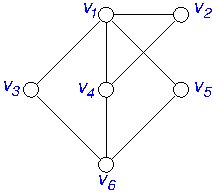
\includegraphics{inputs/col_csp}
      \end{column}
      \begin{column}{2in}
        $V=\{v_1,\dots,v_6\}$\\
        $\bs_1 = (v_1,v_2)$\\
        $\bs_2 = (v_2,v_4)$\\
        % $\bs_3 = (v_1,v_4)$\\
        % $\bs_4=(v_2,v_4)$\\
        \qquad$\vdots$\\
        $\bs_m = (v_5,v_6)$\\[4pt]
        $R_i = R$ for every $i$.
      \end{column}
    \end{columns}
  \end{frame}
\end{comment}

\begin{frame}
  \frametitle{Polymorphisms}

  \begin{exampleblock}{Definition}
    Let $R \in \Rel_k(D)$ and $f\: D^n \to D$. We say 
    \emph{$f$ preserves $R$} if
    \begin{equation*}
      \begin{split}
        (a_{11}, \dots, a_{1k}),&\dots, (a_{n1},\dots, a_{nk}) \in
        R \implies\\ 
        &\bigl( f(a_{11},\dots, a_{n1}), \dots, f(a_{1k},\dots,a_{nk})
        \bigr) \in R
    \end{split}
    \end{equation*}
  \end{exampleblock}
% \end{definition}

  %% \begin{overprint}
  %% \onslide<2|handout:0>
  %% $f$ is an \emph{$n$-ary operation} on $D$.
  %% % 
  %% \onslide<3|handout:1>
    \begin{equation*}
      \newcommand\flab{\scriptstyle{f}}
      \begin{matrix} a_{11} & a_{12} & \dots & a_{1k} & \in & R \\
        a_{21} & a_{22} & \dots & a_{2k} & \in & R \\
        \vdots  & \vdots &       &\vdots  &     & \vdots \\
        a_{n1} & a_{n2} & \dots & a_{nk} & \in & R \\
        %% \downarrow\flab &\downarrow\flab &  & \downarrow\flab \\
        %% \star  & \star  & \dots & \star  & \in & R
        \downarrow &\downarrow &  & \downarrow \\
        (\; f(\ba_1)  & f(\ba_2)  & \dots & f(\ba_k) \; )  & \in & R
      \end{matrix}
    \end{equation*}
  %% \end{overprint}
\end{frame}

\begin{frame}
  \frametitle{Galois Connection}

  % \begin{definition}
  %% \begin{exampleblock}{Definition}
    Let $\sR$ be a set of relations on $D$.

    \bigskip
    \emph{$\Poly(\sR)$}  = set of all operations preserving
    all relations in $\sR$. 

    \bigskip
    These are the \alert{polymorphisms} of  $\sR$. 

    \bigskip

    Let $\sF$ be a set of operations on $D$. 

    \bigskip
    \emph{$\Inv(\sF)$} = set of all relations preserved by all operations in $\sF$.
  %% \end{exampleblock}
% \end{definition}
  
%%   \bigpause
%% Important point: \emph{$(D,\Poly(\sR))$ is an algebraic structure}

\end{frame}

\begin{comment}
  
\begin{frame}
  \begin{exampleblock}{Theorem}
  % \begin{theorem}
    Let $\sS, \sR \sseq \Rel(D)$. Then
    \begin{equation*}
      \Poly(\sS) \sseq \Poly(\sR) \implies \CSP(\sR) \reduc
      \CSP(\sS). 
    \end{equation*}
  \end{exampleblock}

\pause
Thus, the richer the algebraic structure, the easier the corresponding CSP
\end{frame}
\end{comment}

\begin{frame}
\frametitle{Galois Connection...}
  ...from relational to algebraic structures, and back.

  \begin{center}
    \begin{tabular}{ccc}
      \origtextbf{Relational} & &\origtextbf{Algebraic}  \\
      % \origtextbf{Structures} & &\origtextbf{Structures}  \\
      $(D,\sR)$ & $\longrightarrow$ & $(D,\Poly(\sR))$ \\[2pt]
      $(D, \Inv(\sF))$ & $\longleftarrow$ &$(D,\sF)$
    \end{tabular}
  \end{center}

  $\CSP(D,\sR) \equivp \CSP(D,\Inv(\Poly(\sR)))$

  We can use algebra to help classify CSPs!

  \end{frame}



\begin{frame}
  \frametitle{Algebraic CSP}

  For an algebra $\bA = \<A, \sF\>$ \emph{define}
  $\CSP(\A) = \CSP(A, \Inv(\sF))$

  \bigskip

  \begin{exampleblock}{Informal algebraic CSP dichotomy conjecture}

    \bigskip
    If $\Poly(\bA)$ is rich, then $\CSP(\A)$ is tractable.
    
    \bigskip

    If $\Poly(\bA)$ is poor, then $\CSP(\A)$ is \NP-complete.
  \end{exampleblock}

  \pause

  What does it mean to be rich?
  %% Let \A\ and \B\ be algebras

  %% $\B \text{ a subalgebra of \A} \implies \CSP(\B) \reduc \CSP(\A)$.

  %% $\B \text{ a homomorphic image of \A}\implies \CSP(\B) \reduc
  %% \CSP(\A)$. 
  
  %% $\CSP(\A^n) \equivp \CSP(\A)$

\end{frame}


\begin{comment}
  

\begin{frame}
  \begin{exampleblock}{Bulatov, Jeavons, Krokhin, 2000
    \cite{BulatovKrokhinJeavons2000}}
  % \begin{theorem}[Bulatov, Jeavons, Krokhin, 2000
    % \cite{BulatovKrokhinJeavons2000}]
    If $(D,\sR)$ is a ``core'' and every polymorphism is essentially unary,
    then $\CSP(\sR)$ is \NP-complete.
  % \end{theorem}
  \end{exampleblock}

  $f$ is \emph{essentially unary} if $f(x_1,\dots,x_n) = g(x_j)$ for
  some unary $g$ and some $j\leq n$.

 %% \pause
  \begin{exampleblock}{Corollary}
 % \begin{corollary}
    3-COLORABILITY, NONLINEAR SYSTEM, and 3-SAT are \NP-complete.
  % \end{corollary}
  \end{exampleblock}

\end{frame}


\begin{frame}
  \begin{exampleblock}{Bulatov, Larose, Z\'adori, McKenzie, Mar\'oti}
  % \begin{theorem}[Bulatov, Larose, Z\'adori, McKenzie, Mar\'oti
  %   \cite{BulatovJeavonsKrokhin2005,LaroseZadori2003,%
  %   MarotiMcKenzie2008}]
    If $\sR$ is a core and $\Poly(\sR)$ has no WNU operation
    then $\CSP(\sR)$ is \NP-complete.    
  % \end{theorem}
  \end{exampleblock}

  \bigskip
  % \begin{definition}
  \begin{exampleblock}{Definition}
    Let $n>1$. An $n$-ary operation $f$ is called a \emph{weak
      near-unanimity operation} if 
       \begin{equation*}
       \begin{gathered}
       f(x,x,\dots,x) = x \text{ and}\\
    f(y,x,x,x,\dots,x) = f(x,y,x,x,\dots,x) = \cdots\\
    = f(x,x,\dots,x,y)
  \end{gathered}
  \end{equation*}
  % \end{definition}
\end{exampleblock}  
Note: no essentially unary operation is WNU
\end{frame}



\begin{frame}
  \frametitle{Reformuated Dichotomy Conjecture}

  Let $\sR$ be a ``core.''

  $\CSP(\sR)$ is tractable if and only
  if it $\Poly(\sR)$ has a WNU term.

  Otherwise, it is \NP-complete. 

  \bigskip
  \centering{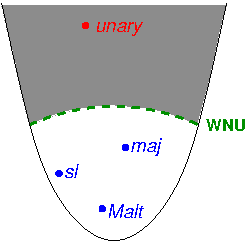
\includegraphics{inputs/dichotomy3}}

\end{frame}

\end{comment}





\begin{frame}
\frametitle{Two General Techniques/Algorithms}
%\begin{enumerate}
\begin{exampleblock}{Method 1}
If $\Poly(\sR)$ contains a ``cube term'' then $\CSP(\sR)\in \P$
%\end{enumerate}
\end{exampleblock}

\pause
Examples of cube terms:

$P(x,y,z) = x-y+z$\\
$M(x,y,z) = \text{majority}$

Algebras with a cube term operation possess ``few subpowers.''

This is used to prove the algorithm is poly-time.

\end{frame}

\begin{frame}
  \frametitle{Two General Techniques for Tractable Algorithms}
\begin{exampleblock}{Method 2}
  If $\Poly(\sR)$ contains WNU terms $v(x,y,z)$ and $w(x,y,z,u)$
  satisfying $v(y,x,x)= w(y,x,x,x)$, then $\CSP(\sR)\in \P$.
\end{exampleblock}

\pause
Examples: majority, semilattice 

Algebras with these operations are congruence $\SD$-$\wedge$

\end{frame}




\begin{frame}
\frametitle{Current State of Affairs}
The two general techniques do not cover all cases of a WNU term. 

\medskip
Two possible directions:

1. Find a completely new algorithm.

2. Combine the two existing algorithms.

We describe some progress in the second direction.
\end{frame}


\begin{frame}
\frametitle{A Motivating Example}
Let $\bA = \<\{0,1,2,3\}, \cdot \>$, have the following Cayley table:

\begin{center}
 \begin{tabular}{c|cccc}
      $\cdot $ & 0 & 1 & 2 & 3\\
      \hline
      0 & 0 & 0 & 3& 2\\
      1 & 0 & 1 & 3& 2\\
      2 & 3 & 3 & 2 & 1\\
      3 & 2 & 2 & 1 & 3
 \end{tabular}
\end{center}

What is an instance of $\CSP(\sansS(\bA))$?

Contraint relations are subdirect products of subalgebras of $\bA$.

The proper nontrivial subuniverses of $\bA$ are $\{0,1\}$ and $\{1,2,3\}$.

\end{frame}

\begin{frame}
  \newcommand{\bS}{\ensuremath{\mathbf{S}}}
  \newcommand{\bSq}{\ensuremath{\mathbf{Sq}}}


  \tikzstyle{lat} = [circle,draw,inner sep=0.8pt]
  \tikzstyle{nodot} = [circle]
  \frametitle{Potatoes of a six-variables instance of $\CSP(\sansS (\bA))$}
  \begin{center}
    \begin{tikzpicture}[scale=1]
          \draw (0,1.5) ellipse (5mm and 26mm);
    \draw (2,1.5) ellipse (5mm and 26mm);
    \draw[blue] (4,2) ellipse (4mm and 18mm);
    \draw[blue] (6,2) ellipse (4mm and 18mm);
    \draw[red] (8,.5) ellipse (4mm and 12mm);
    \draw[red] (10,.5) ellipse (4mm and 12mm);

    \node[nodot] (00) at (0,0) {0};
    \node[nodot] (01) at (0,1) {1};
    \node[nodot] (02) at (0,2) {2};
    \node[nodot] (03) at (0,3) {3};

    \node[nodot] (20) at (2,0) {0};
    \node[nodot] (21) at (2,1) {1};
    \node[nodot] (22) at (2,2) {2};
    \node[nodot] (23) at (2,3) {3};

    \node[nodot] (41) at (4,1) {1};
    \node[nodot] (42) at (4,2) {2};
    \node[nodot] (43) at (4,3) {3};

    \node[nodot] (61) at (6,1) {1};
    \node[nodot] (62) at (6,2) {2};
    \node[nodot] (63) at (6,3) {3};

    \node[nodot] (80) at (8,0) {0};
    \node[nodot] (81) at (8,1) {1};

    \node[nodot] (100) at (10,0) {0};
    \node[nodot] (101) at (10,1) {1};

    %% \node[lat] (00) at (0,0) {};
    %% \node[lat] (01) at (0,1) {};
    %% \node[lat] (20) at (2,0) {};
    %% \node[lat] (21) at (2,1) {};
    %% \node[lat] (41) at (4,1) {};
    %% \node[lat] (42) at (4,2) {};
    %% \node[lat] (43) at (4,3) {};
    %% \node[lat] (61) at (6,1) {};
    %% \node[lat] (62) at (6,2) {};
    %% \node[lat] (63) at (6,3) {};
    %% \node[lat] (80) at (8,0) {};
    %% \node[lat] (81) at (8,1) {};
    %% \node[lat] (82) at (8,2) {};
    %% \node[lat] (83) at (8,3) {};

    %% \draw (00) node [below]{$0$};
    %% \draw (01) node [below]{$1$};
    %% \draw (20) node [below]{$0$};
    %% \draw (21) node [below]{$1$};
    %% \draw (41) node [below]{$1$};
    %% \draw (42) node [below]{$2$};
    %% \draw (43) node [below]{$3$};
    %% \draw (61) node [below]{$1$};
    %% \draw (62) node [below]{$2$};
    %% \draw (63) node [below]{$3$};
    %% \draw (80) node [below]{$0$};
    %% \draw (81) node [below]{$1$};
    %% \draw (82) node [below]{$2$};
    %% \draw (83) node [below]{$3$};


      \draw (0,-1.5) node {$\bA$};
      \draw (2,-1.5) node {$\bA$};
      \draw (4,-1.5) node {$\bSq_3$};
      \draw (6,-1.5) node {$\bSq_3$};
      \draw (8,-1.5) node {$\bS_2$};
      \draw (10,-1.5) node {$\bS_2$};
    \end{tikzpicture}
  \end{center}

\end{frame}





\begin{frame}
  \newcommand{\bS}{\ensuremath{\mathbf{S}}}
  \newcommand{\bSq}{\ensuremath{\mathbf{Sq}}}

\tikzstyle{lat} = [circle,draw,inner sep=0.8pt]
\tikzstyle{nodot} = [circle]
  \frametitle{Subuniverse of Product = Constraint Relation}
  \begin{center}
    \begin{tikzpicture}[scale=.8]
          \draw (0,1.5) ellipse (5mm and 26mm);
    \draw (2,1.5) ellipse (5mm and 26mm);
    \draw (4,2) ellipse (4mm and 18mm);
    \draw (6,2) ellipse (4mm and 18mm);
    \draw (8,.5) ellipse (4mm and 12mm);
    \draw (10,.5) ellipse (4mm and 12mm);

    \node[lat] (00) at (0,0) {};
    \node[lat] (01) at (0,1) {};
    \node[lat] (02) at (0,2) {};
    \node[lat] (03) at (0,3) {};

    \node[lat] (20) at (2,0) {};
    \node[lat] (21) at (2,1) {};
    \node[lat] (22) at (2,2) {};
    \node[lat] (23) at (2,3) {};

    \node[lat] (41) at (4,1) {};
    \node[lat] (42) at (4,2) {};
    \node[lat] (43) at (4,3) {};

    \node[lat] (61) at (6,1) {};
    \node[lat] (62) at (6,2) {};
    \node[lat] (63) at (6,3) {};

    \node[lat] (80) at (8,0) {};
    \node[lat] (81) at (8,1) {};

    \node[lat] (100) at (10,0) {};
    \node[lat] (101) at (10,1) {};


    %% \draw (00) node [below]{$0$};
    %% \draw (01) node [below]{$1$};
    %% \draw (20) node [below]{$0$};
    %% \draw (21) node [below]{$1$};
    %% \draw (41) node [below]{$1$};
    %% \draw (42) node [below]{$2$};
    %% \draw (43) node [below]{$3$};
    %% \draw (61) node [below]{$1$};
    %% \draw (62) node [below]{$2$};
    %% \draw (63) node [below]{$3$};
    %% \draw (80) node [below]{$0$};
    %% \draw (81) node [below]{$1$};
    %% \draw (82) node [below]{$2$};
    %% \draw (83) node [below]{$3$};


      \draw (0,-1.5) node {$\bA$};
      \draw (2,-1.5) node {$\bA$};
      \draw (4,-1.5) node {$\bSq_3$};
      \draw (6,-1.5) node {$\bSq_3$};
      \draw (8,-1.5) node {$\bS_2$};
      \draw (10,-1.5) node {$\bS_2$};
      \draw[green,thick] (00) -- (21) -- (41) -- (63) -- (81) -- (100);
      \draw[yellow,thick] (01) -- (20) -- (42) -- (61) -- (81) -- (101);
      \draw[red,thick] (02) -- (22) -- (43) -- (62) -- (80) -- (100);
      \draw[blue,thick] (03) -- (22) -- (42) -- (63) -- (80) -- (101);
      \draw[pink,thick] (00) -- (23) -- (41) -- (61) -- (80) -- (100);
    \end{tikzpicture}
  \end{center}

  Each colored line represents a tuple in the relation $R$
  
  $R \subseteq A \times A \times Sq_3 \times Sq_3 \times S_2 \times S_2$

  \pause
      {\bf Question:} Does this $R$ form a subuniverse?

\end{frame}

\newcommand{\bB}{\ensuremath{\mathbf{B}}}

\begin{frame}

  \newcommand{\kk}{\ensuremath{\underline{k}}}
\newcommand{\sdp}{\ensuremath{\leq_{\mathrm{sd}}}}


\begin{exampleblock}{Theorem 1}
Let $\bA_i$, $\bB_j$ be finite algebras in a Taylor variety. Assume

\begin{itemize}
\item 
each $\bA_i$ is \alert{abelian}

\item
each $\bB_j$ has a \alert{sink} $s_j$
\end{itemize}

Suppose

  \[
  \bR \sdp \bA_1 \times \cdots \times \bA_J \times \bB_1 \times \cdots \times \bB_K
  \]

  Then
  \[
  \Proj_{1 \dots J}R \times \{s_1\} \times \{s_2\} \times \cdots \times \{s_K\}  \subseteq R
  \]
\end{exampleblock}

By \emph{Taylor variety} we mean an \alert{idempotent} variety with a Taylor term.

\pause

$s\in B$ is called a \alert{sink} if for all
$t \in Clo_k(\bB)$ and $1\leq j \leq k$, if 
$t$ depends on its $j$-th argument, then
$t(b_1, \dots, b_{j-1}, s, b_{j+1}, \dots, b_{k})=s$
for all $b_i \in B$.
\end{frame}


\begin{frame}

  \newcommand{\kk}{\ensuremath{\underline{k}}}
\newcommand{\sdp}{\ensuremath{\leq_{\mathrm{sd}}}}
    
\begin{exampleblock}{Theorem 2}
Let $\bA_i$, $\bB_j$ be finite algebras in a Taylor variety. Assume

\begin{itemize}
\item 
each $\bA_i$ has a \alert{cube term} operation

\item
each $\bB_j$ has a \alert{sink} $s_j$
\end{itemize}

Suppose

  \[
  \bR \sdp \bA_1 \times \cdots \times \bA_J \times \bB_1 \times \cdots \times \bB_K
  \]

  Then
  \[
  \Proj_{1 \dots J}R \times \{s_1\} \times \{s_2\} \times \cdots \times \{s_K\}  \subseteq R
  \]
\end{exampleblock}

\pause

The proof depends on the following result of Barto, Kozik, Stanovsky: a finite idempotent
algebra has a cube term iff every one of its subalgebras has a so called \alert{transitive term
operation}. 
\end{frame}

\begin{frame}
  \frametitle{Application}

  \begin{exampleblock}{Corollary}
  Suppose every algebra in the set $\sA$ contains either a cube terms
  or a sink. Then $\CSP(\sA)$ is tractable.
  \end{exampleblock}
      {\bf Algorithm:}

      Restrict the given instance to potatoes with cube terms.

      Find a solution to the restricted instance (in poly-time by few subpowers).

      If a restricted solution exists, then there is a full solution (by Thm 2).

      If no restricted solution exists, then no full solution exists.
\end{frame}

\begin{frame}
    \frametitle{Quotient strategy}
  Start with
  \[
  \bA_1 \times \bA_2 \times \cdots \times \bA_n
  \]
  Choose a tuple of congruence relations
  \[
  \Theta = (\theta_1, \theta_2,  \dots, \theta_n) \in \prod \Con \bA_i
  \]
  so that $\sA := \{\bA_1/\theta_0, \dots, \bA_n/\theta_n\}$
  is a ``jointly tractable'' set of algebras.

  That is, $\CSP(\sA)$ is tractable.

  {\bf Obvious fact:} a solution to $I$ is a solution to $I/\Theta$.

  For some problems, we have the following converse:

  ({\large $\star$}) a solution to $I/\Theta$ can
  \emph{always} be extended to a solution to $I$. 

  {\bf Problem:} For what algebras does the {\large $\star$}-converse hold?
\end{frame}
\end{document}


\begin{frame}
\frametitle{Back to our motivating example}
Suppose potatoes all come from the set $\{\S_2, \Sq_3\}$.

\begin{exampleblock}{Corollary}
  $\CSP \{\Sq_2, \Sq_3\}$  is tractable
\end{exampleblock}
Solve the instance on the abelian Apply Theorem 1
  
Then we can determine in polynomial time whether a solution exists.

\tikzstyle{lat} = [circle,draw,inner sep=0.8pt]
\begin{frame}
\frametitle{Back to our motivating example}
\begin{center}
  \begin{tikzpicture}[scale=1]
    %%     \draw (0,1.5) ellipse (5mm and 26mm);
    \draw (2,1.5) ellipse (5mm and 26mm);
    \draw (4,2) ellipse (4mm and 18mm);
    \draw (6,2) ellipse (4mm and 18mm);
    \draw (8,.5) ellipse (4mm and 12mm);
    \draw (10,.5) ellipse (4mm and 12mm);

    \node[lat] (00) at (0,0) {};
    \node[lat] (01) at (0,1) {};
    \node[lat] (02) at (0,2) {};
    \node[lat] (03) at (0,3) {};

    \node[lat] (20) at (2,0) {};
    \node[lat] (21) at (2,1) {};
    \node[lat] (22) at (2,2) {};
    \node[lat] (23) at (2,3) {};

    \node[lat] (41) at (4,1) {};
    \node[lat] (42) at (4,2) {};
    \node[lat] (43) at (4,3) {};

    \node[lat] (61) at (6,1) {};
    \node[lat] (62) at (6,2) {};
    \node[lat] (63) at (6,3) {};

    \node[lat] (80) at (8,0) {};
    \node[lat] (81) at (8,1) {};

    \node[lat] (100) at (10,0) {};
    \node[lat] (101) at (10,1) {};


    %% \draw (00) node [below]{$0$};
    %% \draw (01) node [below]{$1$};
    %% \draw (20) node [below]{$0$};
    %% \draw (21) node [below]{$1$};
    %% \draw (41) node [below]{$1$};
    %% \draw (42) node [below]{$2$};
    %% \draw (43) node [below]{$3$};
    %% \draw (61) node [below]{$1$};
    %% \draw (62) node [below]{$2$};
    %% \draw (63) node [below]{$3$};
    %% \draw (80) node [below]{$0$};
    %% \draw (81) node [below]{$1$};
    %% \draw (82) node [below]{$2$};
    %% \draw (83) node [below]{$3$};


    \node[lat] (00) at (0,0) {};
    \node[lat] (01) at (0,1) {};
    \node[lat] (02) at (0,2) {};
    \draw (00) node [right]{$0_A$};
    \draw (01) node [right]{$\theta = 01|2|3$};
    \draw (02) node [right]{$1$};
    \draw (-1.5,1.5) node {$\Con \bA = $};
    \draw[semithick] (00) -- (01) -- (02);

  \end{tikzpicture}
\end{center}
  
\end{frame}





\end{document}


 \hskip1cm
  \begin{tabular}{c|cccc}
      $t$ & 0 & 1 & 2 & 3\\
      \hline
      0 & 0 & 0 & 0& 0\\
      1 & 0 & 1 & 1& 1\\
      2 & 2 & 2 & 2 & 2\\
      3 & 3 & 3 & 3 & 3
    \end{tabular}


\begin{comment}
  
\begin{frame}
\frametitle{The Relational Clone}
For a set $\sR$ of relations on $D$, let $\<\sR\> =
\Inv\bigl(\Poly(\sR)\bigr)$.

$\<\sR\>$ is called the \alert{relational clone} generated by $\sR$.

It coincides with the set of relations definable from $\sR$ by\\
 \emph{primitive positive formulas}.

\pause
$\phi(x_1,\dots,x_n)=(\exists y_1)(\exists y_2)\cdots(\exists y_m)\bigl(R_1(z_{1_1},\dots,z_{1_k}) \meet \dots \meet R_t(z_{t_1},\dots,z_{t_j})\bigr)$

Here $R_1\dots,R_t \in \sR$ and every $z_{i_j} \in \{x_1,\dots,x_n,y_1,\dots,y_m\}$
\end{frame}
\end{comment}



\begin{frame}
  \frametitle{Overcomplicated Definition of CSP}

  $\bA = (A, \sF)$ is a finite idempotent algebra,
  $\Sub(\bA)$ is all subuniverses of $\bA$.

  {\it In this talk} $\CSP(\bA)$ denotes the following decision problem:

   An \alert{instance of degree} $n$ of $\CSP(\bA)$ is the tuple $\<\sV, \sA, \sS, \sR\>$ 
   \begin{itemize}
   \item \emph{variables} $\sV = \{0, 1, \dots, n-1\}$;
   \item \emph{domains} $\sA = \{\bA_0, \bA_1, \dots, \bA_{n-1}\} \subset \Sub(\bA)$  (one for each variable)
   \item \emph{scope functions} $\sS = (\bs_0, \bs_1, \dots, \bs_{p-1})$ 
     with \emph{constraint arities} $\ar(\sS) = (m_0, m_1, \dots, m_{p-1})$
   \item \emph{constraint relations} $\sR = (\bR_0, \bR_1, \dots, \bR_{p-1})$, where
     \[\bR_i \leq \bA_{\bs_i(0)} \times \bA_{\bs_i(1)}\times \cdots \times \bA_{\bs_i(m_i-1)}.\]
   \end{itemize}
 \end{frame}  
 % \bigskip
  
%   A \alert{solution} to $\<\sV, \sA, \sS, \sR\>$ is an assignment
%   $f: \sV \to A$ of values to variables that satisfies all constraints. That is,
%   \[f\in \myprod_{\sV}A_j
%     \quad  \text{and} \quad 
%     \Proj_{\bs_i} f \in \bR_i, \;\text{ for each $0\leq i < p$.}
%   \]

%   \pause
%   {\bf Notation:} $\nn = \{0,1,\dots, n-1\}$, so the $i$-th scope
%   has type $\bs_i : \mm_i \to \nn$ and
%   \[ \Proj_{\bs_i} f  = f \circ \bs_i \]
% \end{frame}





%%% Local Variables: 
%%% mode: latex
%%% TeX-master: t
%%% End: 
